%%%%%%%%%%%%%%%%%%%%%%%%%%%%%%%%%%%%%%%%%%%%%%%%%%%%%%%%%%%%%%%%%%%%%
%%%
%%% Set these variables appropriately
%%%
\newcommand{\AUTHORS}{YOUR NAME HERE}
\newcommand{\TITLE}{PAPER TITLE HERE}
\newcommand{\KEYWORDS}{}
\newcommand{\CONFERENCE}{}
\newcommand{\PAGENUMBERS}{yes}       % "yes" or "no"
\newcommand{\TOAPPEAR}{no}
%%%
%%%
%%%%%%%%%%%%%%%%%%%%%%%%%%%%%%%%%%%%%%%%%%%%%%%%%%%%%%%%%%%%%%%%%%%%%

%%%% Setup the document/page
\documentclass[pdftex,twoside,twocolumn,11pt,letterpaper]{article}
\usepackage{ifthen}

\ifthenelse{\equal{\PAGENUMBERS}{yes}}{%
\usepackage[nohead,
            left=1in,right=1in,top=1in,
            footskip=0.5in,bottom=0.75in     % Room for page numbers
            ]{geometry}
}{%
\usepackage[noheadfoot,columnsep=0.2in,
            margin=1in,centering,truedimen]{geometry}
}

\usepackage{fancyhdr}
\usepackage[numbers,sort]{natbib}
\usepackage{xspace}
\usepackage{booktabs}
\usepackage{subfigure}
\usepackage[T1]{fontenc}
\usepackage{textcomp}
\usepackage{mathptmx}   % Times + Times-like math symbols
\usepackage{courier}
\usepackage[scaled=0.92]{helvet}

\usepackage{color}
\usepackage[pdftex]{graphicx}
\ifthenelse{\isundefined{\wantBW}}{%
  \usepackage[colorlinks]{hyperref}%        % for online version
}{%
  \usepackage[pdfborder={0 0 0}]{hyperref}% % for paper (B&W) version
}
\newcommand{\URL}[1]{\url{#1}}

%%%%% Setup for PDF
\hypersetup{%
pdfauthor = {\AUTHORS},
pdftitle = {\TITLE},
pdfsubject = {\CONFERENCE},
pdfkeywords = {\KEYWORDS},
bookmarksopen = {true}
}

%\setlength{\parindent}{0pt}
%\setlength{\parskip}{0pt}
\renewcommand{\headrulewidth}{0pt}
\newcommand{\Paragraph}[1]{\vspace{-2ex}\paragraph{#1.}}
\setlength{\topmargin}{-.15in}

\ifthenelse{\equal{\PAGENUMBERS}{yes}}{%
  \pagestyle{plain}
}{%
  \pagestyle{empty}
}

\makeatletter\long\def\@makecaption#1#2{
   \vskip 10pt
   \setbox\@tempboxa\hbox{\textsf{#1: #2}}
   \ifdim \wd\@tempboxa >\hsize % IF longer than one line:
       \textsf{#1: #2}\par      % THEN set as ordinary paragraph.
     \else                      % ELSE  center.
       \hbox to\hsize{\hfil\box\@tempboxa\hfil}
   \fi}
\makeatother

\clubpenalty=10000  % Don't allow orphans
\widowpenalty=10000 % Don't allow widows

\title{\textbf{\TITLE}}
\author{\AUTHORS}
\date{}

% Compact itemize and enumerate.  Note that they use the same counters and
% symbols as the usual itemize and enumerate environments.
\def\compactify{\itemsep=0pt \topsep=0pt \partopsep=0pt \parsep=0pt}
\let\latexusecounter=\usecounter
\newenvironment{CompactItemize}
  {\def\usecounter{\compactify\latexusecounter}
   \begin{itemize}}
  {\end{itemize}\let\usecounter=\latexusecounter}
\newenvironment{CompactEnumerate}
  {\def\usecounter{\compactify\latexusecounter}
   \begin{enumerate}}
  {\end{enumerate}\let\usecounter=\latexusecounter}

\newcommand{\comment}[1]{\textcolor{red}{#1}}
\newcommand{\ignore}[1]{}

\newcommand{\xc}[1]{\mbox{\textit{#1}}}
\newcommand{\la}{\leftarrow}
\newcommand{\ra}{\rightarrow}
\newcommand{\somespace}{\hspace{0.1cm}}

\def\discretionaryslash{\discretionary{/}{}{/}}
\def\discretionarydot{\discretionary{.}{}{.}}
\def\discretionarycolon{\discretionary{:}{}{:}}
{\catcode`\/\active
\catcode`\.\active
\catcode`\:\active
\gdef\URLprepare{\catcode`\/\active\let/\discretionaryslash
                 \catcode`\.\active\let.\discretionarydot
                 \catcode`\:\active\let:\discretionarycolon
        \def~{\char`\~}}}%
\def\URL{\bgroup\URLprepare\realURL}%
\def\realURL#1{\tt #1\egroup}%

\newcommand{\eg}{{\em e.g.}, }
\newcommand{\ie}{{\em i.e.}, }
\newcommand{\etal}{{\em et al.\ }}

\def\check{\stackrel{{\scriptscriptstyle ?}}{=}}

\begin{document}
\maketitle

% -*-LaTeX-*-
% $Id: abstract.tex 70 2007-01-30 21:59:16Z nicolosi $
%
% \begin{abstract}

\noindent \large{\textbf{Abstract}}\\
\\
\noindent User passwords are regularly compromised through failures of trusted web servers. Most approaches to solve password problems involve improving server security, improving client practices, or replacing passwords altogether. However, these approaches are not always practical or achievable. In many cases, the undetectable negligence of server owners impedes security improvements. We propose Web Authentication without Transmitting or Storing User Passwords (WATSUP), a new application-layer web protocol to replace standard website authentication, without requiring trust in any server or third party. WATSUP is designed to be auditable, in that a client can always detect if the server incorrectly implements the protocol. WATSUP is secure against eavesdropping and spoofing, even if the communication or server database is compromised. We provide a proof-of-concept implementation of WATSUP, and we discuss the weaknesses and necessary improvements prior to deployment.
% \end{abstract}
   
\section{Introduction}
\label{sec:intro}

Internet users must entrust private information with many different companies, but online security is extremely difficult. Even large and technically advanced companies have lost sensitive information to data breaches and malicious attacks. For example, Yahoo suffered several major breaches in the past few years. First, in 2013 attackers perpetrated the largest recorded data breach when they stole roughly one billion Yahoo accounts \cite{Yahoo_Guardian:2016}.

Then in 2014, a separate attack compromised roughly 500 million Yahoo accounts \cite{Yahoo_CNN:2016}. Neither of these breaches were discovered until 2016, meaning sensitive user information such as hashed passwords and security questions were stolen years before any user became aware.

These types of breaches are not unique to Yahoo \cite{pwned:2016,offenders:2016}. They exemplify a major issue with internet security: users must entrust their personal information to servers and companies that are not transparent, and sometimes not competent, in their implementation of security protocols. Most companies do not publish their full security practices, and even users who are responsible or knowledgeable about online security have no means to verify that their data is being handled correctly. Furthermore, the companies themselves are often unable to detect breaches promptly. As users register for an increasing number of services, the risks described above grow as well.

In spite of the difficulties and flaws of passwords, such as weak user passwords, password reuse, forgetting passwords, and constant breaches of improperly stored passwords, passwords are still unavoidable for users. Despite push from both users and security experts, alternatives rarely catch on, especially in web authentication \cite{microsoft:2011}. Given that passwords have not been eliminated, we focus on improving the security of user passwords, rather than eliminating them entirely.
We propose Web Authentication without Transmitting or Storing User Passwords (WATSUP), a new application-layer protocol that provides users with a transparent, consistent, and easy way to log into a number of different services without trusting any service to properly handle their login credentials. In this paper, we first discuss related work and its drawbacks; next, we propose the WATSUP protocol; third, we discuss a proof-of-concept implementation; and finally, we discuss the advantages and disadvantages of WATSUP and propose future work.

\section{Design}
\label{sec:design}

The standard web login protocol requires the user to input their cleartext password and transmit it to the server, ideally via HTTPS. The WATSUP protocol derives a pseudorandom number generator (PRNG) seed from a key derivation function a user's base password with the hostname and username as a salt. While salting the hostname protects the user against password reuse, salting the username protects against poor server-side salting and hashing. The PRNG is used to generate an asymmetric key pair, which is used to prove identity by decrypting a server-generated nonce.

\begin{figure}
    \centerline{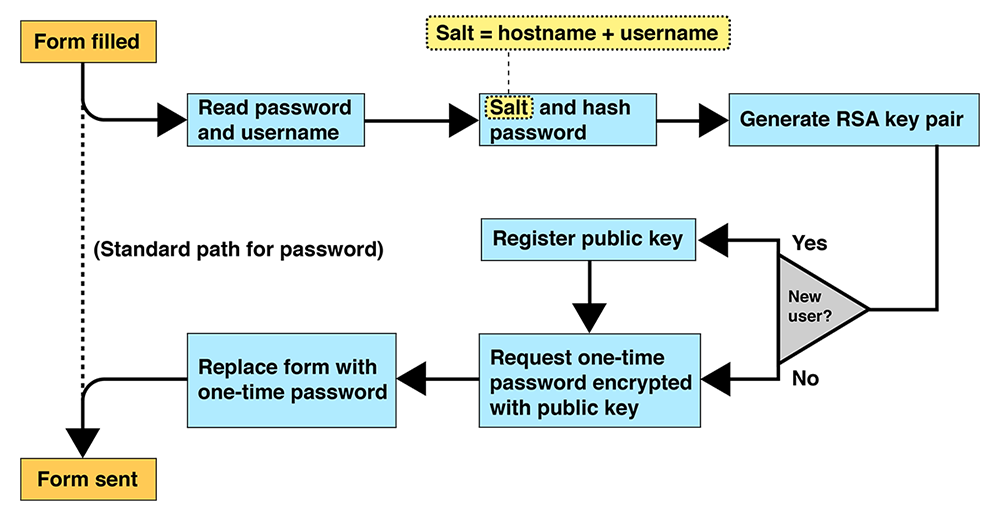
\includegraphics{protocol.png}}
    \caption{Protocol control flow}
\end{figure}

WATSUP generates a unique asymmetric key pair for each site. The key pair is generated with:

\begin{verbatim}
salt = SHA_256(SHA_256(hostname)
               | SHA_256(username))
bits[256] = PBKDF2(root_pass, salt,
                   1000, SHA_256)
prng = seed_ARC4(bits)
key_pair = rsa_key_gen(prng)
\end{verbatim}

Upon registration, the user's public key is stored on the web server. When the user logs in, the server sends the user a cryptographic nonce, encrypted with the user's public key. The WATSUP client uses the generated private key to decrypt the nonce, which it sends to the server as proof of identity.

To support the WATSUP protocol, a server needs to implement the following specifications:

\begin{itemize}

    \item On registration, the server stores the username and associated public key.

    \item On OTP request, generate a cryptographic nonce, associate the nonce with the requesting username, fetch the user's public key, use RSA to encrypt the nonce with the public key, and return the encrypted nonce.

    \item On authentication request, verify the received nonce matches the known nonce. If they match, mark the user as logged in. If not, reject the request.

\end{itemize}





\section{Evaluation}
\label{sec:eval}


\section{Related Work}
\label{sec:related}


\section{Conclusions}
\label{sec:conclusion}

The WATSUP protocol provides usage guarantees for user passwords and reduces the number of points of possible exposure of user passwords. Because the WATSUP protocol never stores or transmits client passwords, users are guaranteed that their cleartext passwords will not be stolen during transit or authentication or from the server. Additionally, this guarantees that remote servers are unable to store cleartext or weakly protected passwords themselves. Users of the WATSUP protocol no longer need to trust a company's security systems to protect their passwords since servers never see cleartext passwords. This mitigates the effect of a data breach.

However, the WATSUP protocol as described in this paper still suffers from some existing security issues. Current common implementations of asymmetric encryption schemes are vulnerable to offline attacks \cite{Blumenthal:2007}. Additionally, if the user chooses a weak base password, the base password may be susceptible to offline dictionary attacks. Both of these attacks are only possible if an attacker obtains a nonce encrypted with a client's public key, or the attacker obtains the public key itself. Even with alternate asymmetric encryption algorithms, the attacker can still perform an offline dictionary attack if they also capture the plaintext nonce; the attack would perform a standard dictionary attack but then generate a public key for each candidate password using the WATSUP's protocol. If any public key decrypts the encrypted nonce and results in the unencrypted nonce, the attack knows the correct password. Alternately, with current encryption schemes, man-in-the-middle attacks are still possible with the WATSUP protocol. It is worth noting that these weaknesses do not expose the client's base password, and would only allow an attacker to impersonate the client when communicating with a single server under a single username. These weaknesses can be eliminated by using HTTPS, but the user still has some guarantees using HTTP.

Another weakness is a Denial of Service attack against the login protocol. An attacker could rapidly request nonces for a target user. Depending on the server implementation, a request may invalidate previous nonces, so the target may be unable to log in.

The WATSUP protocol also does not protect a user from themselves. In order for the WATSUP protocol to provide portable access to online content, a client's private key is reproducible using the client's username and password for a given host. Therefore, if a client loses their password themselves, through some social engineering attack for example, their accounts will still be vulnerable. This also means that online dictionary attacks are still a threat if clients employ weak base passwords. We do not propose WATSUP as a replacement for good password hygiene. Users should still use good practices, such as different passwords on each site and using high entropy passwords.

As discussed in the conclusion, modern asymmetric encryption schemes are not entirely secure. We recommend development and implementation of stronger asymmetric encryption schemes regardless of which authentication model is widely implemented. We also recommend extending the WATSUP protocol. Under the current implementation of WATSUP, users are not able to verify the identity of a server. Extending the protocol to allow for clients and servers to authenticate each other would be beneficial to users. If a client can verify the identity of a server, it can identify insecure situations and refuse to transmit sensitive data. Additionally, the use of HTTPS to secure all communication channels should be enforced whenever possible.

\subsection{Future Work}

Before WATSUP is ready for public use, it needs to be improved and thoroughly vetted by security experts. A major issue that needs to be fixed is the fact that the protocol relies on the server to produce a cryptographic nonce. Our security model does not allow for trust of the server. Therefore, we propose using POSIX time in milliseconds as a nonce. As long as the ping is greater than one millisecond, and the server is correctly providing the time, this nonce will be unique, and hence adequate for cryptographic use. The client can then audit the server's compliance by ensuring the client's POSIX time and the server's POSIX time match within some generous delta (e.g. 1 day). This could cause an issue if the client's clock is not accurate.

Another pathway that could be explored is that of mutual authentication---a trust-on-first-use system could be put in place. This would provide server authenticity guarantees to the user, which could be critical in the event of HTTPS PKI compromise. To solve this, one model is that the user saves the server's public key, but this means trust will need to be reestablished on each new device. Another model is that the user signs the server's public key, which the server saves and reissues to the user on each connection, but this makes revocation in the event of server compromise difficult or impossible. In either model, the server would perform authentication similar to the client authentication.

As previously discussed, WATSUP is vulnerable to offline dictionary attacks against the base password, since attackers can observe both the encrypted nonce and decrypted nonce. Additionally, properties of asymmetric encryption mean that access to just the encrypted nonce is sufficient for an offline attack. With better cryptography, the WATSUP protocol may be able to avoid these issues by never revealing the encrypted nonce in the first place. Tunneling WATSUP through a secure channel, such as HTTPS, already solves this. However, in situations where HTTPS is not available, it is still important to try to protect users. Any solution needs to follow the core ideas of WATSUP: it must be simple for the server to implement, and it must not rely on trusting the server.

%% Bibliography
%\vspace{-1ex}
%\linespread{1.0}
%\setlength{\bibsep}{1pt}
%\footnotesize
\small
\bibliography{local}
\bibliographystyle{abbrvnat}

\end{document}

